%% LyX 1.6.8 created this file.  For more info, see http://www.lyx.org/.
%% Do not edit unless you really know what you are doing.
\documentclass[oneside,english,american,pdftex, a4paper, twoside, BCOR12mm, titlepage, openright, headsepline, chapterprefix, mpexclude,  idxtotoc, liststotoc, cleardoublestandard]{scrbook}
\usepackage[T1]{fontenc}
\usepackage[latin9]{inputenc}
\setcounter{secnumdepth}{3}
\setcounter{tocdepth}{3}
\setlength{\parskip}{\medskipamount}
\setlength{\parindent}{0pt}
\usepackage{color}
\usepackage{array}
\usepackage{verbatim}
\usepackage{float}
\usepackage{amsmath}
\usepackage{amssymb}
\usepackage{esint}

\makeatletter

%%%%%%%%%%%%%%%%%%%%%%%%%%%%%% LyX specific LaTeX commands.
%% Because html converters don't know tabularnewline
\providecommand{\tabularnewline}{\\}
\floatstyle{ruled}
\newfloat{algorithm}{tbp}{loa}[chapter]
\floatname{algorithm}{Algorithm}

%%%%%%%%%%%%%%%%%%%%%%%%%%%%%% Textclass specific LaTeX commands.
\floatstyle{ruled}
\newfloat{algorithm}{tbp}{loa}
\floatname{algorithm}{Algorithm}
\usepackage[noend]{algorithmic}
\newcommand{\forbody}[1]{ #1 \ENDFOR}
\newcommand{\ifbody}[1]{ #1  \ENDIF}
\newcommand{\whilebody}[1]{ #1  \ENDWHILE}
\renewcommand{\algorithmicprint}{\textbf{draw}}

%%%%%%%%%%%%%%%%%%%%%%%%%%%%%% User specified LaTeX commands.


\usepackage{euscript}

\DeclareSymbolFont{rsfscript}{OMS}{rsfs}{m}{n}
\DeclareSymbolFontAlphabet{\mathrsfs}{rsfscript}


% PDF formatting instructions for A4
\pdfpagewidth=210mm % for pdflatex
\pdfpageheight=296mm % for pdflatex



%%%%%%%% begin tikz %%%%%%
\usepackage{tikz,tkz-base}
\usetikzlibrary{shapes,decorations,shadows}
\usetikzlibrary{decorations.pathmorphing}
\usetikzlibrary{decorations.shapes}
\usetikzlibrary{fadings}
\usetikzlibrary{patterns}
\usetikzlibrary{calc}
\usetikzlibrary{decorations.text}
\usetikzlibrary{decorations.footprints}
\usetikzlibrary{decorations.fractals}
\usetikzlibrary{shapes.gates.logic.IEC}
\usetikzlibrary{shapes.gates.logic.US}
\usetikzlibrary{fit,chains}
\usetikzlibrary{positioning}
\usepgflibrary{shapes}
\usetikzlibrary{scopes}
\usetikzlibrary{arrows}
\usetikzlibrary{backgrounds}

\tikzset{latent/.style={circle,fill=white,draw=black,inner sep=1pt, 
minimum size=20pt, font=\fontsize{10}{10}\selectfont},
obs/.style={latent,fill=gray!25},
const/.style={rectangle, inner sep=0pt},
factor/.style={rectangle, fill=black,minimum size=5pt, inner sep=0pt},
>={triangle 45}}


\pgfdeclarelayer{b}
\pgfdeclarelayer{f}
\pgfsetlayers{b,main,f}

% shapename, fitlist, caption, pos
\newcommand{\plate}[4]{
\begin{pgfonlayer}{b}
\node (invis#1) [draw, color=white, inner sep=2pt,rectangle,fit=#2] {};
\end{pgfonlayer}\begin{pgfonlayer}{f}
\node (capt#1) [ below left=0 pt of invis#1.south east, xshift=2pt,yshift=1pt] {\footnotesize{#3}};
\node (#1) [draw,inner sep=1pt, rectangle,fit=(invis#1) (capt#1),#4] {};
\end{pgfonlayer}
}


\newcommand{\shiftedplate}[5]{
\begin{pgfonlayer}{b}
\node (invis#1) [draw, color=white, inner sep=0 pt,rectangle,fit=#2] {};
\end{pgfonlayer}\begin{pgfonlayer}{f}
\node (capt#1) [#5, xshift=2pt] {\footnotesize{#3}};
\node (#1) [draw,inner sep=2pt, rectangle,fit=(invis#1) (capt#1),#4] {};
\end{pgfonlayer}
}

%shapename, pos, caption, in1, in2, out, captpos
\newcommand{\twofactor}[7]{
\node (#1) [factor] at #2 {};
\node (capt#1) [#7 of #1]{\footnotesize{#3}};
\draw [-] (#4) -- (#1) ;
\draw [-] (#5) -- (#1) ;
\draw [->,thick] (#1) -- (#6);
}

%shapename, pos, caption, in, out, captpos
\newcommand{\factor}[6]{
\node (#1) [factor] at #2 {};
\node (capt#1) [#6 of #1]{\footnotesize{#3}};
\draw [-] (#4) -- (#1) ;
\draw [->,thick] (#1) -- (#5);
}

% name, --, caption, pos
\newcommand{\nofactor}[4]{
\node (#1) [factor, #2]  {};
\node (capt#1) [#4 of #1]{\footnotesize{#3}};
}

%shapename,  fitlist, caption
\newcommand{\namedgate}[3]{
\begin{pgfonlayer}{b}
\node (invisgate#1) [rectangle, draw, color=white,  fit=#2] {};
\end{pgfonlayer}
\node (gatecapt#1) [ above right=0 pt of invisgate#1.north west, xshift=-1pt ] {\footnotesize{#3}};
\node (#1) [rectangle,draw,dashed, inner sep=2pt, fit=(invisgate#1)(gatecapt#1)]{};

}

%shapename,  fitlist, caption
\newcommand{\gate}[3]{
\node (#1) [rectangle,draw,dashed, inner sep=2pt, fit=#2]{};
}

%shapename,  fitlist1, fitlist2, caption1, caption2
\newcommand{\vertgate}[5]{
\begin{pgfonlayer}{b}
\node (invisgateleft#1) [rectangle, draw, color=white,  fit=#2] {};
\node (invisgateright#1) [rectangle, draw, color=white,  fit=#4] {};
\end{pgfonlayer}
\node (gatecaptleft#1) [ above left=0 pt of invisgateleft#1.north east, xshift=1pt ]{\footnotesize{#3}};
\node (gatecaptright#1) [ above right=0 pt of invisgateright#1.north west, xshift=-1pt ] {\footnotesize{#5}};
\node (#1) [rectangle,draw,dashed, inner sep=2pt, fit=(invisgateleft#1)(gatecaptleft#1)(invisgateright#1)(gatecaptright#1)]{};
\draw [-, dashed] (#1.north) -- (#1.south);
}


\newcommand{\vertgateSpec}[5]{
\begin{pgfonlayer}{b}
\node (invisgateleft#1) [rectangle, draw, color=white,  fit=#2] {};
\node (invisgateright#1) [rectangle, draw, color=white,  fit=#4] {};
\end{pgfonlayer}
\node (gatecaptleft#1) [ above left=0 pt of invisgateleft#1.north east, xshift=1pt ]{\footnotesize{#3}};
\node (gatecaptright#1) [ above right=0 pt of invisgateright#1.north west, xshift=-1pt ] {\footnotesize{#5}};
\node (#1) [rectangle,draw,dashed, inner sep=2pt, fit=(invisgateleft#1)(gatecaptleft#1)(invisgateright#1)(gatecaptright#1)]{};
\draw [-, dashed] (#1.70) -- (#1.290);
}

\newcommand{\horgate}[5]{
\begin{pgfonlayer}{b}
\node (invisgateleft#1) [rectangle, draw, color=white,  fit=#2] {};
\node (invisgateright#1) [rectangle, draw, color=white,  fit=#4] {};
\end{pgfonlayer}
\node (gatecaptleft#1) [ above right=0 pt of invisgateleft#1.south west, xshift=1pt ]{\footnotesize{#3}};
\node (gatecaptright#1) [ below right=0 pt of invisgateright#1.north west, xshift=-1pt ] {\footnotesize{#5}};
\node (#1) [rectangle,draw,dashed, inner sep=2pt, fit=(invisgateleft#1)(gatecaptleft#1)(invisgateright#1)(gatecaptright#1)]{};
\draw [-, dashed] (#1.west) -- (#1.east);
}

\newcommand{\horogate}[5]{
\begin{pgfonlayer}{b}
\node (invisgateleft#1) [rectangle, draw, color=white,  fit=#2] {};
\node (invisgateright#1) [rectangle, draw, color=white,  fit=#4] {};
\end{pgfonlayer}
\node (#1) [rectangle,draw,dashed, inner sep=2pt, fit=(invisgateleft#1)(invisgateright#1)]{};
\node (gatecaptleft#1) [ above right=0 pt of #1.west, xshift=0pt ]{\footnotesize{#3}};
\node (gatecaptright#1) [ below right=0 pt of #1.west, xshift=0pt ] {\footnotesize{#5}};

\draw [-, dashed] (#1.west) -- (#1.east);
}


\newcommand{\vertogate}[5]{
\begin{pgfonlayer}{b}
\node (invisgateleft#1) [rectangle, draw, color=white,  fit=#2] {};
\node (invisgateright#1) [rectangle, draw, color=white,  fit=#4] {};
\end{pgfonlayer}
\node (#1) [rectangle,draw,dashed, inner sep=2pt, fit=(invisgateleft#1)(invisgateright#1)]{};
\node (gatecaptleft#1) [ below left=0 pt of #1.north, xshift=0pt ]{\footnotesize{#3}};
\node (gatecaptright#1) [ below right=0 pt of #1.north, xshift=0pt ] {\footnotesize{#5}};

\draw [-, dashed] (#1.north) -- (#1.south);
}


%%%%%%%% end tikz %%%%%%

\makeatother

\usepackage{babel}

\begin{document}

\title{Probabilistic Models in Tikz}


\author{Laura Dietz}

\maketitle
Tikz macros and examples for probabilistic models. I use the directed
factor graph notation in most figures, but you can use the same macros
to draw Bayesian networks.

\selectlanguage{english}%
\global\long\def\items{\EuScript{V}}


\global\long\def\tastes{\CMcal{T}}


\global\long\def\nodes{\EuScript{N}}


\global\long\def\edges{\EuScript{E}}


\global\long\def\content{\mathrsfs{C}}


\global\long\def\vocab{\CMcal{V}}


\global\long\def\docs{\CMcal{D}}


\global\long\def\cites{\CMcal{C}}


\global\long\def\up#1{\uppercase{#1}}



\chapter{Foundations}

%
\begin{figure}[H]
\noindent \begin{centering}
\begin{tabular}{cc}
%
\begin{comment}
p(X|Z,R,Q)\textbackslash{}cdot p(R|Z,Q)\textbackslash{}cdot p(Z|Q)\textbackslash{}cdot
p(Q)
\end{comment}
{}

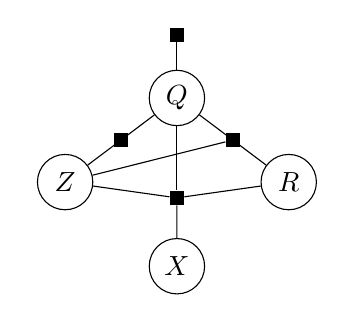
\begin{tikzpicture}
\node [matrix,matrix anchor=mid, column sep=20pt, row sep=10pt] {
&\node (q) [latent] {$Q$};&\\
\node (z) [latent] {$Z$};
&\node (qrzx) [factor,below=3pt] {};&
\node (r) [latent] {$R$};\\
&\node (x) [latent] {$X$};&\\
};

\node (qfac) [factor, above=10pt of q] {};
\draw [-] (q) -- (qfac);

\draw [-] (q) -- (z) node (qz) [midway,factor] {};
\draw [-] (q) -- (r) node (qrz) [midway,factor] {};
\draw [-] (qrz) -- (z);

\draw [-] (r) -- (qrzx) -- (x);
\draw [-] (z) -- (qrzx);
\draw [-] (q) -- (qrzx);


\end{tikzpicture} & %
\begin{comment}
p(X|Z)\textbackslash{}cdot p(Z|Q)\textbackslash{}cdot p(R|Q)\textbackslash{}cdot
p(Q)
\end{comment}
{}

\noindent \centering{}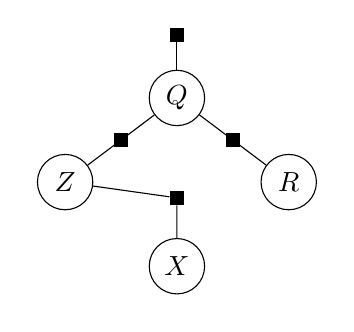
\begin{tikzpicture}
\node [matrix,matrix anchor=mid, column sep=20pt, row sep=10pt] {
&\node (q) [latent] {$Q$};&\\
\node (z) [latent] {$Z$};
&\node (qrzx) [factor,below=3pt] {};&
\node (r) [latent] {$R$};\\
&\node (x) [latent] {$X$};&\\
};

\node (qfac) [factor, above=10pt of q] {};
\draw [-] (q) -- (qfac);

\draw [-] (q) -- (z) node (qz) [midway,factor] {};
\draw [-] (q) -- (r) node (qrz) [midway,factor] {};


\draw [-] (z) -- (qrzx) -- (x);

\end{tikzpicture}\tabularnewline
a) & b)\tabularnewline
\end{tabular}
\par\end{centering}

\caption[Factor graphs for visualizing factorizations of a joint distribution.]{Factor graphs for visualizing factorizations of a joint distribution
$p(X,Z,R,Q)$. a) General factorization, b) Factorization with conditional
independence assumptions.\label{fig:Factorization}}

\end{figure}


%
\begin{figure}[H]
\noindent \begin{centering}
\begin{tabular}{cc}
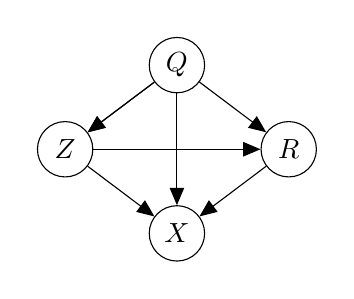
\begin{tikzpicture}
\node [matrix,matrix anchor=mid, column sep=20pt, row sep=10pt] {
&\node (q) [latent] {$Q$};&\\
\node (z) [latent] {$Z$};
&&
\node (r) [latent] {$R$};\\
&\node (x) [latent] {$X$};&\\
};

\draw [->] (q) -- (z) ;
\draw [->] (q) -- (r) ;
\draw [->] (q) -- (z);

\draw [->] (z) -- (r);

\draw [->] (r) -- (x);
\draw [->] (z) -- (x);
\draw [->] (q) -- (x);


\end{tikzpicture} & \noindent \begin{centering}
%
\begin{comment}
p(X|Z)\textbackslash{}cdot p(Z|Q)\textbackslash{}cdot p(R|Q)\textbackslash{}cdot
p(Q)
\end{comment}
{}
\par\end{centering}

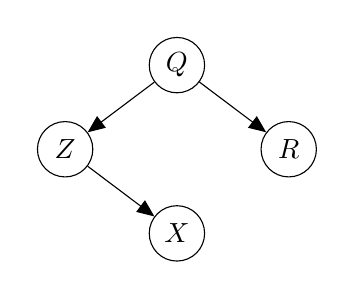
\begin{tikzpicture}
\node [matrix,matrix anchor=mid, column sep=20pt, row sep=10pt] {
&\node (q) [latent] {$Q$};&\\
\node (z) [latent] {$Z$};
&&
\node (r) [latent] {$R$};\\
&\node (x) [latent] {$X$};&\\
};

\draw [->] (q) -- (z) ;
\draw [->] (q) -- (r) ;


\draw [->] (z)  -- (x);

\end{tikzpicture}\tabularnewline
a) & b)\tabularnewline
\end{tabular}
\par\end{centering}

\caption{Bayesian network visualization for factor graphs in Figure \ref{fig:Factorization}.\label{fig:bayes}}

\end{figure}


%
\begin{figure}[H]
\noindent \begin{centering}
\begin{tabular}{cc}
%
\begin{comment}
p(X|Z,R,Q)\textbackslash{}cdot p(R|Z,Q)\textbackslash{}cdot p(Z|Q)\textbackslash{}cdot
p(Q)
\end{comment}
{}

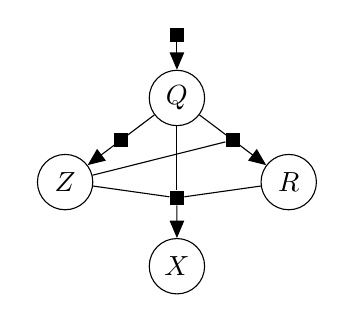
\begin{tikzpicture}
\node [matrix,matrix anchor=mid, column sep=20pt, row sep=10pt] {
&\node (q) [latent] {$Q$};&\\
\node (z) [latent] {$Z$};
&\node (qrzx) [factor,below=3pt] {};&
\node (r) [latent] {$R$};\\
&\node (x) [latent] {$X$};&\\
};

\node (qfac) [factor, above=10pt of q] {};
\draw [->] (qfac) -- (q);

\draw [->] (q) -- (z) node (qz) [midway,factor] {};
\draw [->] (q) -- (r) node (qrz) [midway,factor] {};
\draw [-] (qrz) -- (z);

\draw [->] (r) -- (qrzx) -- (x);
\draw [-] (z) -- (qrzx);
\draw [-] (q) -- (qrzx);


\end{tikzpicture} & %
\begin{comment}
p(X|Z)\textbackslash{}cdot p(Z|Q)\textbackslash{}cdot p(R|Q)\textbackslash{}cdot
p(Q)
\end{comment}
{}

\noindent \centering{}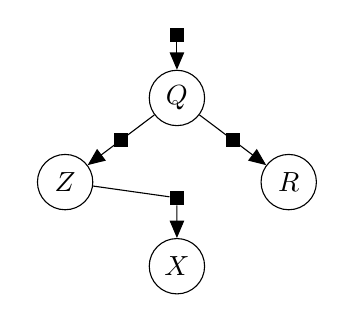
\begin{tikzpicture}
\node [matrix,matrix anchor=mid, column sep=20pt, row sep=10pt] {
&\node (q) [latent] {$Q$};&\\
\node (z) [latent] {$Z$};
&\node (qrzx) [factor,below=3pt] {};&
\node (r) [latent] {$R$};\\
&\node (x) [latent] {$X$};&\\
};

\node (qfac) [factor, above=10pt of q] {};
\draw [->] (qfac) -- (q);

\draw [->] (q) -- (z) node (qz) [midway,factor] {};
\draw [->] (q) -- (r) node (qrz) [midway,factor] {};


\draw [->] (z) -- (qrzx) -- (x);

\end{tikzpicture}\tabularnewline
a) & b)\tabularnewline
\end{tabular}
\par\end{centering}

\caption{Directed factor graph visualization for factor graphs in Figure \ref{fig:Factorization}.\label{fig:dir-factorgraph}}

\end{figure}


%
\begin{figure}[H]
\noindent \begin{centering}
\begin{tabular}{cc}
%
\begin{comment}
gate: Z=z

p(X|Y) p(R|Z)

gate Z!=z

p(X,R|Z)
\end{comment}
{}

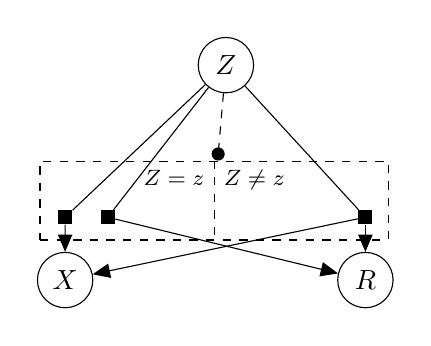
\begin{tikzpicture}
\node [matrix,matrix anchor=mid, column sep=30pt, row sep=10pt] {

&\node (z) [latent] {$Z$};&
\\[20pt,between borders]

\node (xz) [factor] {};
\node (rz) [factor,right = 10 pt of xz] {};
\node (spacexz) [rectangle, draw, transparent,  above = 5pt of xz] {};
&& \node (rzx) [factor] {};
\\

\node (x) [latent] {$X$};
&& \node (r) [latent] {$R$};
\\
};

\draw [->] (z) -- (xz) -- (x);
\draw [->] (z) -- (rz) -- (r);
\draw [->] (z) -- (rzx) -- (x);
\draw [->] (rzx) -- (r);

%shapename,  fitlist1, fitlist2, caption1, caption2
\vertogate{g}{(xz)(rz)(spacexz)}{$Z=z$}{(rzx)}{$Z\neq z$};

\draw [-*,dashed] (z) -- (g);
\end{tikzpicture} & %
\begin{comment}
gate Q=0

p(X|R)

gate Q=1

p(X|Z)
\end{comment}
{}

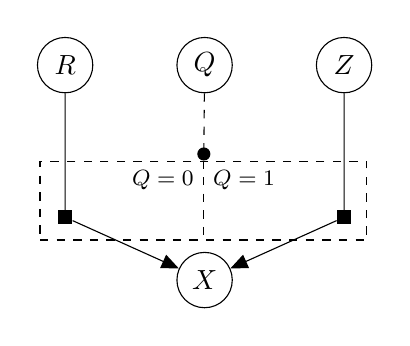
\begin{tikzpicture}
\node [matrix,matrix anchor=mid, column sep=30pt, row sep=10pt] {

\node (r) [latent] {$R$};
&\node (q) [latent] {$Q$};
&\node (z) [latent] {$Z$};
\\[20pt,between borders]

\node (xr) [factor] {};
\node (spacexr) [rectangle, draw, transparent,  above = 5pt of xr] {};
&& \node (xz) [factor] {};
\\

&\node (x) [latent] {$X$};
&
\\
};

\draw [->] (r) -- (xr) -- (x);
\draw [->] (z) -- (xz) -- (x);

%shapename,  fitlist1, fitlist2, caption1, caption2
\vertogate{g}{(xr)(spacexr)}{$Q=0$}{(xz)}{$Q=1$};
\draw [-*,dashed] (q) -- (g);
\end{tikzpicture}\tabularnewline
a) & b)\tabularnewline
\end{tabular}
\par\end{centering}

\caption[Representing context-specific independence by gates in factor graphs.]{Representing context-specific independence by gates (dashed boxes)
in factor graphs.\label{fig:factors-and-gates}}

\end{figure}


%
\begin{figure}[H]
\noindent \begin{centering}
\begin{tabular}{c}
%
\begin{comment}
p(theta)

plate: i=1..n

p(X|theta )
\end{comment}
{}

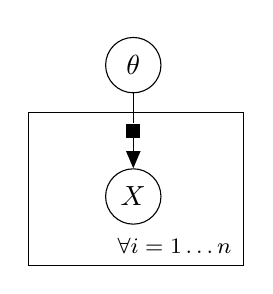
\begin{tikzpicture}
\node [matrix,matrix anchor=mid, column sep=30pt, row sep=10pt] {

\node (theta) [latent] {$\theta$};
\\

\node (xtheta) [factor] {};
\node (spaceleft) [rectangle, draw, transparent,  left = 25pt of xtheta] {};
\node (spaceright) [rectangle, draw, transparent,  right = 25pt of xtheta] {};
\\

\node (x) [latent] {$X$};
\\
};
\plate{p}{(xtheta)(spaceleft)(spaceright)(x)}{$\forall i=1\ldots n$}{}

\draw [->] (theta) -- (xtheta) -- (x);

\end{tikzpicture}\tabularnewline
\end{tabular}
\par\end{centering}

\caption[Representing repetition of connection templates by plates in factor
graphs.]{Representing repetition of connection templates by plates (solid
boxes) in factor graphs.\label{fig:plates}}

\end{figure}


%
\begin{figure}[H]
\noindent \begin{centering}
\begin{tabular}{c}
%
\begin{comment}
p(theta|alpha, beta)

plate: i=1..n

p(X|theta )
\end{comment}
{}

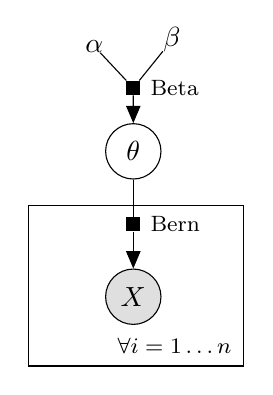
\begin{tikzpicture}
\node [matrix,matrix anchor=mid, column sep=30pt, row sep=10pt] {

\node (theta) [latent] {$\theta$};
\\

\nofactor{xtheta}{}{Bern}{right=0pt};

\node (spaceleft) [rectangle, draw, transparent,  left = 25pt of xtheta] {};
\node (spaceright) [rectangle, draw, transparent,  right = 25pt of xtheta] {};
\\

\node (x) [obs] {$X$};
\\
};
\plate{p}{(xtheta)(spaceleft)(spaceright)(x)}{$\forall i=1\ldots n$}{}

\draw [->] (theta) -- (xtheta) -- (x);

\nofactor{drawtheta}{above=10pt of theta}{Beta}{right=0pt};
\node (alpha) [const, above left=10pt and 8 pt of drawtheta]  {$\alpha$};
\node (beta) [const, above right=10pt and 8 pt of drawtheta]  {$\beta$};

\draw [->] (alpha) -- (drawtheta) -- (theta);
\draw [-] (beta) -- (drawtheta);


\end{tikzpicture}\tabularnewline
\end{tabular}
\par\end{centering}

\caption{Beta-Bernoulli example with hyperparameters.\label{fig:beta-bernoulli-example-hyperparams}}

\end{figure}



\section{Latent Dirichlet Allocation}

\selectlanguage{american}%
%
\begin{figure}[H]
\selectlanguage{english}%
\noindent \begin{centering}
% Latent Dirichlet allocation
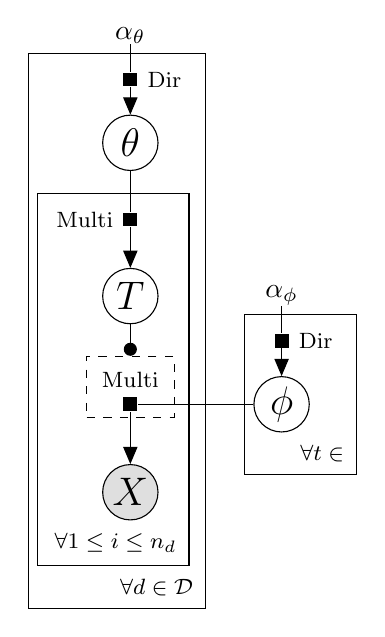
\begin{tikzpicture}
[latent/.style={circle,fill=white,draw=black,inner sep=1pt, minimum size=20pt, font=\fontsize{14}{14}\selectfont},
obs/.style={latent,fill=gray!25},
const/.style={rectangle, inner sep=0pt}]


\matrix[row sep=4mm,column sep=10mm, matrix anchor=mid] (lda) {
&

\\

&

\\

\node (lambda) [latent] {$\theta$}; 
&

\\

\nofactor{drawtc}{}{Multi}{left=0pt};
&

\\

\node (tc) [latent]  {$T$}; 
&

\\

\nofactor{drawxc}{}{Multi}{above=0pt}; \gate{gatexc}{(drawxc) (captdrawxc)}{$t$};
&  \node (phi) [latent]  {$\phi$};

\\

\node (xc) [obs]  {$X$}; 
&

\\
};


\nofactor{drawlambda}{above=10pt of lambda}{Dir}{right=0pt};
\nofactor{drawphi}{above=10pt of phi}{Dir}{right=0pt};


\node (alphalambda) [const, above=10pt of drawlambda]  {$\alpha_{\theta}$};
\node (alphaphi) [const, above=10pt of drawphi]  {$\alpha_{\phi}$};

\draw [->] (alphaphi) -- (drawphi) -- (phi);
\draw [->] (alphalambda) -- (drawlambda) -- (lambda);




\draw [->] (lambda) -- (drawtc) -- (tc);
\draw [->] (phi) -- (drawxc) -- (xc);


\draw [-*] (tc) -- (gatexc);



\plate{contentplatec}{(tc)(xc)(drawtc)(drawxc)(captdrawtc)(captdrawxc)(gatexc)}{$\forall 1 \leq i \leq n_d  $}{}
\plate{userplatec}{(contentplatec)(lambda)(drawlambda)(captdrawlambda)}{$\forall d \in \mathcal{D}$}{}

\plate{topicplate}{(phi)(drawphi)(captdrawphi)}{$\forall t \in \tastes$}{}


\end{tikzpicture}

\par\end{centering}

\selectlanguage{american}%
\caption{Latent Dirichlet allocation as directed factor graph.\label{fig:lda-factorgraph}}

\end{figure}



\chapter{Citation Influence Model}


\section{Plain Citation Influence Model}

%
\begin{figure}[H]
\selectlanguage{english}%
\noindent \begin{centering}
% Citation Influence
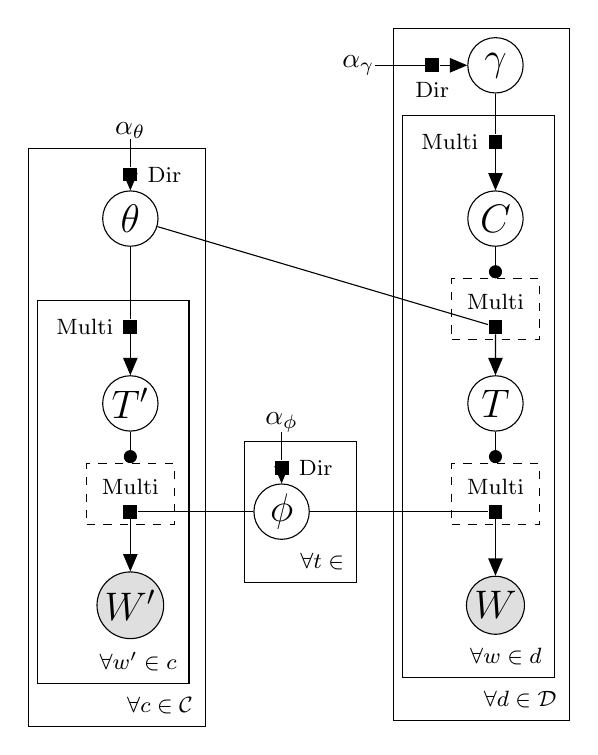
\begin{tikzpicture}
[latent/.style={circle,fill=white,draw=black,inner sep=1pt, minimum size=20pt, font=\fontsize{14}{14}\selectfont},
obs/.style={latent,fill=gray!25},
const/.style={rectangle, inner sep=0pt}]


\matrix[row sep=4mm,column sep=10mm, matrix anchor=mid] (citinf) {
&
&[3mm] \node (psi) [latent] {$\gamma$}; 
\\

&
& \nofactor{drawf}{}{Multi}{left=0pt};
\\

\node (lambda) [latent] {$\theta$}; 
&
& \node (f) [latent]  {$C$}; 
\\

\nofactor{drawtc}{}{Multi}{left=0pt};
&
& \nofactor{drawtd}{}{Multi}{above=0pt};\gate{gatetd}{(drawtd) (captdrawtd)}{$\tastes$};
\\

\node (tc) [latent]  {$T'$}; 
&
& \node (td) [latent]  {$T$}; 
\\

\nofactor{drawxc}{}{Multi}{above=0pt}; \gate{gatexc}{(drawxc) (captdrawxc)}{$t$};
&  \node (phi) [latent]  {$\phi$};
& \nofactor{drawxd}{}{Multi}{above=0pt}; \gate{gatexd}{(drawxd) (captdrawxd)}{$t$};
\\

\node (xc) [obs]  {$W'$}; 
&
&\node (xd) [obs]  {$W$}; \\
\\
};

\nofactor{drawpsi}{left=10pt of psi}{Dir}{below=0pt};
\nofactor{drawlambda}{above=3pt of lambda}{Dir}{right=0pt};
\nofactor{drawphi}{above=3pt of phi}{Dir}{right=0pt};

\node (alphapsi) [const, left=18pt of drawpsi] {$\alpha_{\gamma}$}; 
\node (alphalambda) [const, above=10pt of drawlambda]  {$\alpha_{\theta}$};
\node (alphaphi) [const, above=10pt of drawphi]  {$\alpha_{\phi}$};

\draw [->] (alphaphi) -- (drawphi) -- (phi);
\draw [->] (alphalambda) -- (drawlambda) -- (lambda);
\draw [->] (alphapsi) -- (drawpsi) -- (psi);


\draw [->] (psi) -- (drawf) -- (f);
\draw [->] (lambda) -- (drawtc) -- (tc);
\draw [->] (lambda) -- (drawtd) -- (td);
\draw [->] (phi) -- (drawxc) -- (xc);
\draw [->] (phi) -- (drawxd) -- (xd);

\draw [-*] (tc) -- (gatexc);
\draw [-*] (td) -- (gatexd);
\draw [-*] (f) -- (gatetd);

\plate{contentplatec}{(tc)(xc)(drawtc)(drawxc)(captdrawtc)(captdrawxc)(gatexc)}{$\forall w' \in c$}{}
\plate{userplatec}{(contentplatec)(lambda)(drawlambda)(captdrawlambda)}{$\forall c \in \mathcal{C}$}{}
\plate{contentplated}{(f)(td)(xd)(drawtd)(drawxd)(drawf)(captdrawtd)(captdrawxd)(captdrawf)(gatetd)(gatexd)}{$\forall w \in d$}{}
\plate{userplated}{(contentplated)(psi)(drawpsi)(captdrawpsi)}{$\forall d \in \mathcal{D}$}{}

\plate{topicplate}{(phi)(drawphi)(captdrawphi)}{$\forall t \in \tastes$}{}


\end{tikzpicture}

\par\end{centering}

\selectlanguage{american}%
\caption{Citation influence model in directed factor graph notation.\label{fig:Citinf-plain-model}}

\end{figure}


%
\begin{algorithm}[H]
%
\begin{algorithmic}
[1]\selectlanguage{english}%
\FORALL{$t\in\tastes$}

\forbody{\PRINT{$\phi_{t}\sim\mbox{Dir}(\alpha_{\phi})$}}

\FORALL{$c\in\mathcal{C}$ as cited role}

\forbody{\PRINT{$\theta_{c}\sim\mbox{Dir}(\alpha_{\theta})$}

\STATE{// Generate content $w$ according to LDA:}

\FORALL{words $w_{c,i}'\in c$}

\forbody{\PRINT{topic $\up t'_{c,i}\sim\mbox{Multi}(\theta_{c})$}

\PRINT{word $\up w'_{c,i}\sim\mbox{Multi}(\phi_{\up t'_{c,i}})$}}}

\FORALL{$d\in\mathcal{D}$ as citing role}

\forbody{\PRINT{$\gamma_{d}\sim\mbox{Dir}(\alpha_{\gamma})$}

\FORALL{words $w_{d,i}\in d$}

\forbody{\PRINT{citation $\up c_{d,i}\sim\mbox{Multi}(\gamma_{d})$}\label{Flo:dedication-begin}

\PRINT{topic $\up t_{d,i}\sim\mbox{Multi}(\theta_{\up c_{d,i}})$}

\PRINT{word $\up w_{d,i}\sim\mbox{Multi}(\phi_{\up t_{d,i}})$}\label{Flo:dedication-end}}}\selectlanguage{american}

\end{algorithmic}


\caption[Generative process of the plain citation influence model.]{Generative process of the plain citation influence model. For a description
of each variable see Table \ref{tab:Variable-description-plain}.\label{alg:Citinf-plain}}

\end{algorithm}


%
\begin{table}[H]
\caption[Notation for the plain citation influence model.]{Notation for the plain citation influence model. Variables in the
cited plate are denoted with prime.}


\label{tab:Variable-description-plain}

{\small }\begin{tabular}{|>{\centering}p{0.11\linewidth}|>{\raggedright}p{0.79\linewidth}|}
\hline 
{\small Symbol} & {\small Description}\tabularnewline
\hline
\hline 
{\small $\up c$, $c$} & {\small cited publication}\tabularnewline
\hline 
{\small $d$} & {\small citing publication}\tabularnewline
\hline 
{\small $\theta$} & {\small shared topic mixture associated with a cited publication}\tabularnewline
\hline 
{\small $\phi$} & {\small characteristic word distribution for each topic}\tabularnewline
\hline 
{\small $\gamma$} & {\small distribution of citation influences}\tabularnewline
\hline 
{\small $\up w$', $\up w$} & {\small words in cited, citing publications respectively}\tabularnewline
\hline 
{\small $\up t$', $\up t$} & {\small topic assignments of tokens in cited, citing publications
respectively}\tabularnewline
\hline 
{\small $\alpha$} & {\small Dirichlet / beta parameters of the multinomial / Bernoulli
distributions}\tabularnewline
\hline
\end{tabular}
\end{table}



\section{Citation Influence Model with Own Topics}

%
\begin{figure}[H]
\selectlanguage{english}%
\noindent \begin{centering}
% Citation Influence
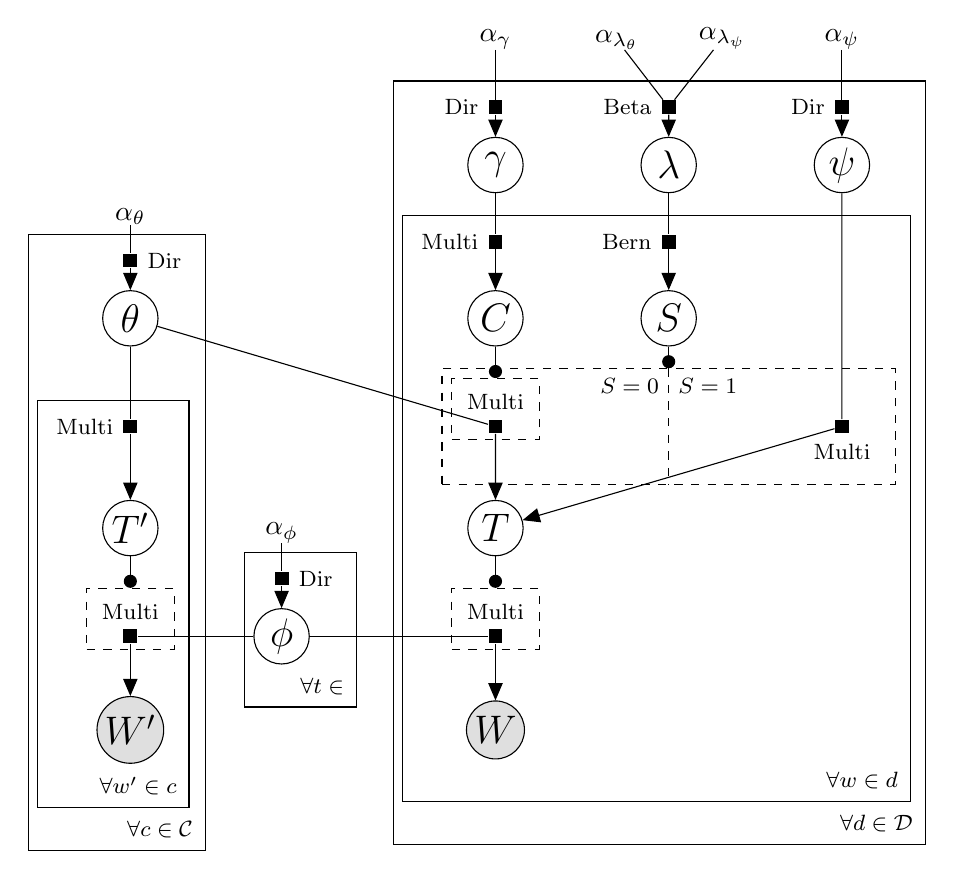
\begin{tikzpicture}
[latent/.style={circle,fill=white,draw=black,inner sep=1pt, minimum size=20pt, font=\fontsize{14}{14}\selectfont},
obs/.style={latent,fill=gray!25},
const/.style={rectangle, inner sep=0pt}]


\matrix[row sep=4mm,column sep=10mm, matrix anchor=mid] (citinf) {
&
&[3mm] \node (psi) [latent] {$\gamma$};
&[12mm,between origins] \node (balance) [latent] {$\lambda$};
&[12mm,between origins] \node (innov) [latent] {$\psi$};
\\

&
& \nofactor{drawf}{}{Multi}{left=0pt};
&\nofactor{drawbalance}{}{Bern}{left=0pt};
&
\\

\node (lambda) [latent] {$\theta$}; 
&
& \node (f) [latent]  {$C$}; 
&\node (s) [latent]  {$S$}; 
&
\\

\nofactor{drawtc}{}{Multi}{left=0pt};
&
& \nofactor{drawtd}{}{Multi}{above=0pt};\gate{gatetd}{(drawtd) (captdrawtd)}{$\tastes$};
&
&\nofactor{drawtdinnov}{}{Multi}{below=0pt};
\\

\node (tc) [latent]  {$T'$}; 
&
& \node (td) [latent]  {$T$}; 
&
&
\\

\nofactor{drawxc}{}{Multi}{above=0pt}; \gate{gatexc}{(drawxc) (captdrawxc)}{$t$};
&  \node (phi) [latent]  {$\phi$};
& \nofactor{drawxd}{}{Multi}{above=0pt}; \gate{gatexd}{(drawxd) (captdrawxd)}{$t$};
&
&
\\

\node (xc) [obs]  {$W'$}; 
&
&\node (xd) [obs]  {$W$}; 
&
&
\\
\\
};

\vertogate{gates}{(drawtd)(captdrawtd)}{$S=0$}{(drawtdinnov)(captdrawtdinnov)}{$S=1$};

\nofactor{drawlambda}{above=8pt of lambda}{Dir}{right=0pt};
\node (alphalambda) [const, above=10pt of drawlambda]  {$\alpha_{\theta}$};

\nofactor{drawphi}{above=8pt of phi}{Dir}{right=0pt};
\node (alphaphi) [const, above=10pt of drawphi]  {$\alpha_{\phi}$};

\nofactor{drawpsi}{above=8pt of psi}{Dir}{left=0pt};
\node (alphapsi) [const, above=18pt of drawpsi] {$\alpha_{\gamma}$}; 

\nofactor{drawbalancep}{above=8pt of balance}{Beta}{left=0pt};
\node (alphabalance1) [const, above left=18pt and 8 pt of drawbalancep] {$\alpha_{\lambda_{\theta}}$}; 
\node (alphabalance2) [const, above right=18pt and 8 pt of drawbalancep] {$\alpha_{\lambda_{\psi}}$}; 

\nofactor{drawinnovp}{above=8pt of innov}{Dir}{left=0pt};
\node (alphainnov) [const, above=18pt of drawinnovp] {$\alpha_{\psi}$}; 

\draw [->] (alphaphi) -- (drawphi) -- (phi);
\draw [->] (alphalambda) -- (drawlambda) -- (lambda);
\draw [->] (alphapsi) -- (drawpsi) -- (psi);
\draw [->] (alphabalance1) -- (drawbalancep) -- (balance);
\draw [-] (alphabalance2) -- (drawbalancep);
\draw [->] (alphainnov) -- (drawinnovp) -- (innov);

\draw [->] (psi) -- (drawf) -- (f);
\draw [->] (lambda) -- (drawtc) -- (tc);
\draw [->] (lambda) -- (drawtd) -- (td);
\draw [->] (phi) -- (drawxc) -- (xc);
\draw [->] (phi) -- (drawxd) -- (xd);
\draw [->] (balance) -- (drawbalance) -- (s);
\draw [->] (innov) -- (drawtdinnov) -- (td);


\draw [-*] (tc) -- (gatexc);
\draw [-*] (td) -- (gatexd);
\draw [-*] (f) -- (gatetd);
\draw [-*] (s) -- (gates);


\plate{contentplatec}{(tc)(xc)(drawtc)(drawxc)(captdrawtc)(captdrawxc)(gatexc)}{$\forall w' \in c$}{}
\plate{userplatec}{(contentplatec)(lambda)(drawlambda)(captdrawlambda)}{$\forall c \in \mathcal{C}$}{}
\plate{contentplated}{(f)(td)(xd)(drawtd)(drawxd)(drawf)(captdrawtd)(captdrawxd)(captdrawf)(gatetd)(gatexd)(gates)(s)(drawbalance)}{$\forall w \in d$}{}
\plate{userplated}{(contentplated)(psi)(drawpsi)(captdrawpsi)(balance)(drawbalance)(captdrawbalance)(innov)}{$\forall d \in \mathcal{D}$}{}

\plate{topicplate}{(phi)(drawphi)(captdrawphi)}{$\forall t \in \tastes$}{}


\end{tikzpicture}

\par\end{centering}

\selectlanguage{american}%
\caption{Citation influence model with own topics as directed factor graph.\label{fig:Citinf-owntopics-model}}

\end{figure}


%
\begin{algorithm}[H]
%
\begin{algorithmic}
[1]\selectlanguage{english}%
\FORALL{$t\in\tastes$}

\forbody{\PRINT{$\phi_{t}\sim\mbox{Dir}(\alpha_{\phi})$ ranging over the vocabulary
$\vocab$.}}

\FORALL{cited $c\in\mathcal{C}$}

\forbody{\PRINT{topic mixture $\theta_{c}\sim\mbox{Dir}(\alpha_{\theta})$ ranging
over topics $\tastes$.}

\STATE{// Generate content $w$ according to LDA:}

\FORALL{words $w_{c,i}\in c$}

\forbody{\PRINT{topic $\up t'_{c,i}\sim\mbox{Multi}(\theta_{c})$}

\PRINT{word $\up w'_{c,i}\sim\mbox{Multi}(\phi_{\up t'_{c,i}})$}}}

\FORALL{citing $d\in\mathcal{D}$ }

\forbody{\PRINT{$\gamma_{d}\sim\mbox{Dir}(\alpha_{\gamma})$ ranging over $L(d)$.}

\PRINT{$\lambda_{d}\sim\mbox{Beta}(\alpha_{\lambda_{\theta}},\alpha_{\lambda_{\psi}})$}

\PRINT{$\psi_{d}\sim\mbox{Dir}(\alpha_{\psi})$ ranging over topics $\tastes$.}

\FORALL{words $w_{d,i}\in d$}

\forbody{\PRINT{coin toss $\up s_{d,i}\sim\mbox{Bern}(\lambda_{d})$}

\selectlanguage{american}%
\IF{$\up s_{d,i}=0$}

\ifbody{\selectlanguage{english}%
\STATE{// Generate token by inheritance:}

\PRINT{a cited publication $\up c_{d,i}\sim\mbox{Multi}(\gamma_{d})$.}\label{Flo:inherit-begin}

\PRINT{topic $\up t_{d,i}\sim\mbox{Multi}(\theta_{\up c_{d,i}})$ \foreignlanguage{american}{from
the cited document's topic mixture.}}\label{Flo:inherit-end}

\selectlanguage{american}%
\ELSIF{$\up s_{d,i}=1$}

\selectlanguage{english}%
\STATE{// Generate token by innovation:}\label{Flo:innov-begin}

\PRINT{topic $\up t_{d,i}\sim\mbox{Multi}(\psi_{d})$ from the own topic
mixture.}\label{Flo:innov-end}\selectlanguage{american}
}

\selectlanguage{english}%
\PRINT{word $\up w_{d,i}\sim\mbox{Multi}(\phi_{\up t_{d,i}})$}}}\selectlanguage{american}

\end{algorithmic}


\caption{Generative process of the citation influence model with own topics.\label{alg:Citinf-owntopics}}

\end{algorithm}


%
\begin{table}[tb]
\caption{Further notation used in the citation influence model with own topics.}


\label{tab:Variable-description-owntopics}

{\small }\begin{tabular}{|>{\centering}p{0.11\linewidth}|>{\raggedright}p{0.79\linewidth}|}
\hline 
{\small Symbol} & {\small Description}\tabularnewline
\hline
\hline 
{\small $\psi$} & {\small innovation topic mixture of a citing publication}\tabularnewline
\hline 
{\small $\lambda$} & {\small parameter of the coin flip, choosing to draw topics from $\theta$
or $\psi$}\tabularnewline
\hline 
{\small $\up s$} & {\small indicates whether the topic of a citing publication is drawn
from inheritance or innovation}\tabularnewline
\hline
\end{tabular}
\end{table}



\chapter{Shared Taste Model}


\section{Plain Shared Taste Model}

%
\begin{table}[H]
\noindent \begin{centering}
\begin{tabular}{|>{\centering}p{0.2\textwidth}|>{\raggedright}p{0.7\textwidth}|}
\hline 
Symbol & Description\tabularnewline
\hline
\hline 
$\lambda_{\{u,f\}}$ & Shared topic mixture associated with the undirected edge between users
$u$ and $f$.\tabularnewline
\hline 
$T$ & Topic for items.\tabularnewline
\hline 
$\phi$ & Item distribution for each topic.\tabularnewline
\hline 
\selectlanguage{english}%
$\psi_{u}$\selectlanguage{american}
 & Distribution over friends of user $u$ according to their strength
of influence on the user's content.\tabularnewline
\hline 
$F$ & Friend associated with an observed item (if not explained by {}``own
topics'').\tabularnewline
\hline 
$X$ & Observed item in contents of the user.\tabularnewline
\hline 
$\Omega_{u}$ & Background topic mixture of the user (the own topics). Alternatively
a mixture over own items.\tabularnewline
\hline 
$\epsilon$ & Coin parameter deciding on how much content of the user is explained
by the {}``own topics''\tabularnewline
\hline 
$E$ & Boolean indicator, if 1, the observed item is explained by the {}``own
topics'' rather than the shared topics.\tabularnewline
\hline
\end{tabular}
\par\end{centering}

\caption{Notation for shared taste model with own topics.\label{tab:Notation-shared-taste}}

\end{table}


%
\begin{figure}[H]
\selectlanguage{english}%
\noindent \begin{centering}
% Shared Taste Model
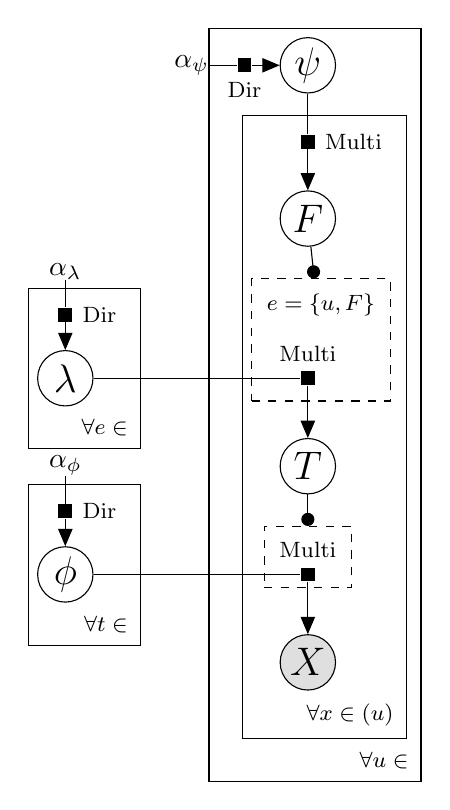
\begin{tikzpicture}
[latent/.style={circle,fill=white,draw=black,inner sep=1pt, minimum size=20pt, font=\fontsize{14}{14}\selectfont},
obs/.style={latent,fill=gray!25},
const/.style={rectangle, inner sep=0pt}]




\matrix[row sep=4mm,column sep=10mm, matrix anchor=mid] (sharedtaste) {

& 
& \node (psi) [latent] {$\psi$}; 
\\

&
& \nofactor{drawf}{}{Multi}{right=0pt};
\\

& 
& \node (f) [latent]  {$F$}; 
\\

\node (lambda) [latent] {$\lambda$};
& 
& \nofactor{drawt}{}{Multi}{above=0pt};\namedgate{gatet}{(drawt) (captdrawt)}{$e=\{u,F\}$};
\\

& 
& \node (t) [latent]  {$T$}; 
\\

\node (phi) [latent]  {$\phi$};
& 
& \nofactor{drawx}{}{Multi}{above=0pt}; \gate{gatex}{(drawx) (captdrawx)}{$t$};
\\

& 
& \node (x) [obs]  {$X$}; \\
};

\nofactor{drawpsi}{left=10pt of psi}{Dir}{below=0pt};
\nofactor{drawlambda}{above=10pt of lambda}{Dir}{right=0pt};
\nofactor{drawphi}{above=10pt of phi}{Dir}{right=0pt};

\node (alphapsi) [const, left=10pt of drawpsi] {$\alpha_{\psi}$}; 
\node (alphalambda) [const, above=10pt of drawlambda]  {$\alpha_{\lambda}$};
\node (alphaphi) [const, above=10pt of drawphi]  {$\alpha_{\phi}$};

\draw [->] (alphaphi) -- (drawphi) -- (phi);
\draw [->] (alphalambda) -- (drawlambda) -- (lambda);
\draw [->] (alphapsi) -- (drawpsi) -- (psi);

\draw [->] (psi) -- (drawf) -- (f);
\draw [->] (lambda) -- (drawt) -- (t);
\draw [->] (phi) -- (drawx) -- (x);

\draw [-*] (t) -- (gatex);
\draw [-*] (f) -- (gatet);

\plate{contentplate}{(f)(t)(x)(drawt)(drawx)(drawf)(captdrawt)(captdrawx)(captdrawf)(gatet)(gatex)}{$\forall x \in \content (u)$}{}
\plate{userplate}{(contentplate)(psi)(drawpsi)(captdrawpsi)}{$\forall u \in \nodes$}{}
\plate{topicplate}{(phi)(drawphi)(captdrawphi)}{$\forall t \in \tastes$}{}
\plate{edgeplate}{(lambda)(drawlambda)(captdrawlambda)}{$\forall e \in \edges$}{}


\end{tikzpicture}

\par\end{centering}

\selectlanguage{american}%
\caption{Shared taste model as directed factor graph.\label{fig:sharedtaste-model-factorgraph}}

\end{figure}


%
\begin{algorithm}[H]
%
\begin{algorithmic}
[1]\selectlanguage{english}%
\FORALL{$t\in\mathcal{T}$}

\forbody{\PRINT{$\phi_{t}\sim\mbox{Dir}(\alpha_{\phi})$}}

\FORALL{$\{u,f\}\in\mathcal{E}$}

\forbody{\PRINT{shared topic mixture $\lambda_{\{f,u\}}=\lambda_{\{u,f\}}\sim\mbox{Dir}(\alpha_{\lambda})$.}\label{Flo:sparse-topic-prior}}

\FORALL{$u\in\mathcal{N}$}

\forbody{\PRINT{friend mixture $\psi_{u}\sim\mbox{Dir}(\alpha_{\psi})$ ranging over
friends of $u$.}

\FORALL{items $x_{u,i}\in\mathcal{C}(u)$}\forbody{\PRINT{friend $F_{u,i}\sim\mbox{Multi}(\psi_{u})$}

\PRINT{topic $T_{u,i}\sim\mbox{Multi}(\lambda_{\{u,F_{u,i}\}})$}

\PRINT{item $X_{u,i}\sim\mbox{Multi}(\phi_{T_{u,i}})$}}}\selectlanguage{american}

\end{algorithmic}


\caption{\selectlanguage{english}%
Generative process of the shared taste model.\label{alg:Shared-Taste-Model}\selectlanguage{american}
}

\end{algorithm}



\section{Shared Taste Model with Own Topics}

%
\begin{algorithm}[H]
%
\begin{algorithmic}
[1]\selectlanguage{english}%
\FORALL{$t\in\mathcal{T}$}

\forbody{\PRINT{$\phi_{t}\sim\mbox{Dir}(\alpha_{\phi})$}}

\FORALL{$\{u,f\}\in\mathcal{E}$}

\forbody{\PRINT{shared topic mixture $\lambda_{\{f,u\}}=\lambda_{\{u,f\}}\sim\mbox{Dir}(\alpha_{\lambda})$.}}

\FORALL{$u\in\mathcal{N}$}

\forbody{\PRINT{friend mixture $\psi_{u}\sim\mbox{Dir}(\alpha_{\psi})$ ranging over
friends of $u$.}

\PRINT{background distribution $\Omega_{u}\sim\mbox{Dir}(\alpha_{\Omega})$}

\PRINT{background coin $\epsilon_{u}\sim\mbox{Beta}(a_{\epsilon},b_{\epsilon})$}

\FORALL{item $x_{u,i}\in\mathcal{C}(u)$}\forbody{\PRINT{coin flip $E_{u,i}\sim\mbox{Bern}(\epsilon_{u})$}

\IF{$E_{u,i}=0$}

\ifbody{\STATE{// Generate from shared topic.}

\PRINT{friend $F_{u,i}\sim\mbox{Multi}(\psi_{u})$}

\PRINT{topic $T_{u,i}\sim\mbox{Multi}(\lambda_{\{u,F_{u,i}\}})$ from share
topics}

\ELSIF{$E_{u,i}=1$}

\STATE{// Generate from background.}

\PRINT{topic $T_{u,i}\sim\mbox{Multi}(\Omega_{u})$ from own topics}}

\PRINT{item $X_{u,i}\sim\mbox{Multi}(\phi_{T_{u,i}})$}}}\selectlanguage{american}

\end{algorithmic}


\caption{\selectlanguage{english}%
Generative process of the shared taste model with own topics.\label{alg:Shared-Taste-Model-own-topics}\selectlanguage{american}
}

\end{algorithm}


%
\begin{figure}[H]
\selectlanguage{english}%
\noindent \begin{centering}
% Shared Taste Model own topics
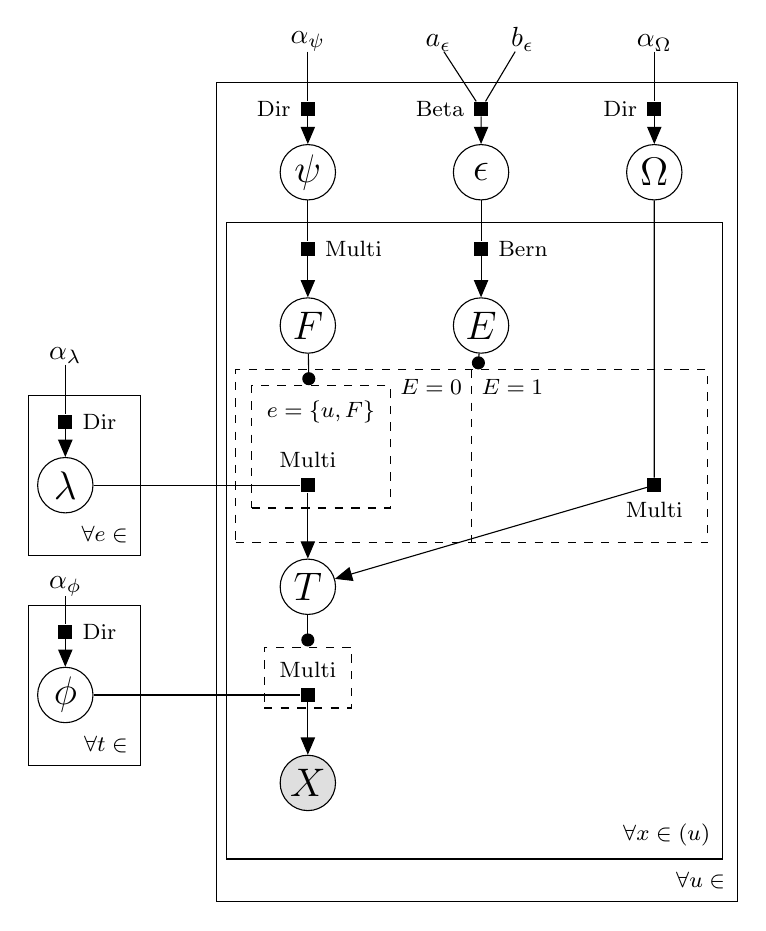
\begin{tikzpicture}
[latent/.style={circle,fill=white,draw=black,inner sep=1pt, minimum size=20pt, font=\fontsize{14}{14}\selectfont},
obs/.style={latent,fill=gray!25},
const/.style={rectangle, inner sep=0pt}]




\matrix[row sep=4mm,column sep=10mm, matrix anchor=mid] (sharedtaste) {

& 
& \node (psi) [latent] {$\psi$}; 
&[12mm,between origins] \node (balance) [latent] {$\epsilon$};
&[12mm,between origins] \node (innov) [latent] {$\Omega$};
\\

&
& \nofactor{drawf}{}{Multi}{right=0pt};
& \nofactor{drawe}{}{Bern}{right=0pt};
& 
\\

& 
& \node (f) [latent]  {$F$}; 
& \node (e) [latent]  {$E$}; 
& 
\\


\node (lambda) [latent] {$\lambda$};
& 
& \nofactor{drawt}{}{Multi}{above=0pt};\namedgate{gatet}{(drawt) (captdrawt)}{$e=\{u,F\}$};
&
&\nofactor{drawtinnov}{}{Multi}{below=0pt};
\\

& 
& \node (t) [latent]  {$T$}; 
&
&
\\

\node (phi) [latent]  {$\phi$};
& 
& \nofactor{drawx}{}{Multi}{above=0pt}; \gate{gatex}{(drawx) (captdrawx)}{$t$};
&
&
\\

& 
& \node (x) [obs]  {$X$}; 
&
& 
\\
};

\vertogate{gates}{(gatet)}{$E=0$}{(drawtinnov)(captdrawtinnov)}{$E=1$};


\nofactor{drawpsi}{above=10pt of psi}{Dir}{left=0pt};
\nofactor{drawlambda}{above=10pt of lambda}{Dir}{right=0pt};
\nofactor{drawphi}{above=10pt of phi}{Dir}{right=0pt};
\nofactor{drawbalance}{above=10pt of balance}{Beta}{left=0pt};
\nofactor{drawinnov}{above=10pt of innov}{Dir}{left=0pt};

\node (alphapsi) [const, above=18pt of drawpsi] {$\alpha_{\psi}$}; 
\node (alphalambda) [const, above=18pt of drawlambda]  {$\alpha_{\lambda}$};
\node (alphaphi) [const, above=10pt of drawphi]  {$\alpha_{\phi}$};
\node (abalance) [const, above left=18pt and 8 pt of drawbalance]  {$a_{\epsilon}$};
\node (bbalance) [const, above right=18pt and 8 pt of drawbalance]  {$b_{\epsilon}$};
\node (alphainnov) [const, above=18pt of drawinnov]  {$\alpha_{\Omega}$};



\draw [->] (alphaphi) -- (drawphi) -- (phi);
\draw [->] (alphalambda) -- (drawlambda) -- (lambda);
\draw [->] (alphapsi) -- (drawpsi) -- (psi);
\draw [->] (alphainnov) -- (drawinnov) -- (innov);
\draw [->] (abalance) -- (drawbalance) -- (balance);
\draw [-] (bbalance) -- (drawbalance);

\draw [->] (psi) -- (drawf) -- (f);
\draw [->] (lambda) -- (drawt) -- (t);
\draw [->] (phi) -- (drawx) -- (x);
\draw [->] (balance) -- (drawe) -- (e);
\draw [->] (innov) -- (drawtinnov) -- (t);

\draw [-*] (t) -- (gatex);
\draw [-*] (f) -- (gatet.101);
\draw [-*] (e) -- (gates);

\plate{contentplate}{(gates)(drawe)(f)(t)(x)(drawt)(drawx)(drawf)(captdrawt)(captdrawx)(captdrawf)(gatet)(gatex)}{$\forall x \in \content (u)$}{}
\plate{userplate}{(contentplate)(psi)(drawpsi)(captdrawpsi)(drawbalance)(captdrawbalance)(drawinnov)(captdrawinnov)}{$\forall u \in \nodes$}{}
\plate{topicplate}{(phi)(drawphi)(captdrawphi)}{$\forall t \in \tastes$}{}
\plate{edgeplate}{(lambda)(drawlambda)(captdrawlambda)}{$\forall e \in \edges$}{}


\end{tikzpicture}

\par\end{centering}

\selectlanguage{american}%
\caption{Shared taste model with own topics as directed factor graph.\label{fig:sharedtaste-owntopics-model-factorgraph}}

\end{figure}



\section{Pairwise Link LDA model (Nallapati 08)}

The original pairwise Link LDA model (Nallapati, Ahmed, Xing, Cohen.
Joint latent topic models for text and citations, KDD, 2008) is modified
to correct for rarity of interactions (Airoldi, Blei, Fienberg, Xing.
Mixed membership stochastic blockmodels, JMLR, 2008).

%
\begin{figure}[H]
\selectlanguage{english}%
\noindent \begin{centering}
% Pairwise Link LDA model (Nallapati 08)
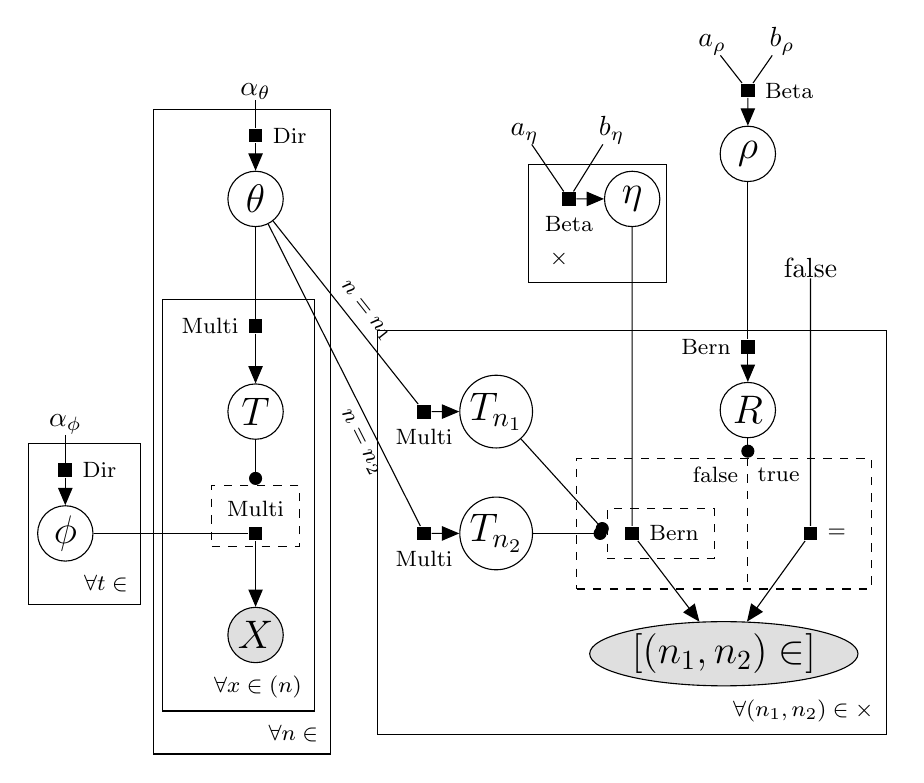
\begin{tikzpicture}
[latent/.style={circle,fill=white,draw=black,inner sep=1pt, minimum size=20pt, font=\fontsize{14}{14}\selectfont},
obs/.style={latent,fill=gray!25},
const/.style={rectangle, inner sep=0pt}]

%[10mm,between origins]  
\node [matrix,row sep=4mm,column sep=4mm, matrix anchor=mid]  (blockmodel) {
&[6mm]
&[7mm] 
&[5mm]
& 
&
\\

& \node (theta) [latent] {$\theta$}; 
&
& \node (eta) [latent] {$\eta$}; 
& 
&
\\

&
&
&
& \node (false) [const,xshift=7mm] {false};
& 
\\

& \nofactor{drawtd}{}{Multi}{left=0pt}; 
& 
& 
& 
&
\\

& \node (td) [latent] {$T$};
& \nofactor{drawtu}{}{Multi}{below=0pt}; \node (tu) [latent,right=10pt of drawtu] {$T_{n_1}$};
& 
& 
& 
\\

\node (phi) [latent]  {$\phi$};
& \nofactor{drawxd}{}{Multi}{above=0pt}; \gate{gatexd}{(drawxd) (captdrawxd)}{$t$};
& \nofactor{drawtf}{}{Multi}{below=0pt}; 
\node (tf) [latent, right=10pt of drawtf] {$T_{n_2}$}; 
&  \nofactor{drawedge}{}{Bern}{right=0pt}; 
\node (drawedgeborder)[fit=(drawedge),outer sep=1pt]{};
\gate{gateedge}{(drawedgeborder)(drawedge) (captdrawedge)}{$t_{n_1}\rightarrow t_{n_2}$};
& \nofactor{drawfalse}{xshift=7mm}{=}{right=0pt};
& 
\\

& \node (xd) [obs] {$X$};
&
&
& \node (edgeobs) [transparent]{};
&
\\
};

\node (gateedgeborder) [fit=(gateedge),outer sep=2pt]{};

\vertgateSpec{gateback}{(drawedge)(gateedge)(gateedgeborder)(captdrawedge)}{}{(drawfalse)(captdrawfalse)}{};
\node [below left=0pt of gateback.70]{\footnotesize{$\textrm{false}$}};
\node [below right=0pt of gateback.70]{\footnotesize{$\textrm{true}$}};

\node (e) [latent, above=7pt of gateback.70] {$R$};
\nofactor{drawe}{above=10pt of e}{Bern}{left=0pt};
\node (edge) [obs, ellipse,below=4mm of gateback.south]  {$[(n_1,n_2)\in \edges]$};


\node (rho) [latent, above=35mm of gateback.70] {$\rho$};  

\nofactor{draweta}{left=10pt of eta}{Beta}{below=0pt};
\nofactor{drawtheta}{above=10pt of theta}{Dir}{right=0pt};
\nofactor{drawphi}{above=10pt of phi}{Dir}{right=0pt};
\nofactor{drawrho}{above=10pt of rho}{Beta}{right=0pt};

\begin{scope}[node distance=17pt and 8pt]
  \node (alphaeta) [const, above left= of draweta] {$a_{\eta}$}; 
  \node (b-eta) [const, above right= of draweta] {$b_{\eta}$}; 
\end{scope}
\begin{scope}[node distance=10pt and 5pt]
   \node (alpharho) [const, above left= of drawrho] {$a_{\rho}$}; 
  \node (b-rho) [const, above right= of drawrho] {$b_{\rho}$}; 
\end{scope}
\node (alphatheta) [const, above=10pt of drawtheta]  {$\alpha_{\theta}$};
\node (alphaphi) [const, above=10pt of drawphi]  {$\alpha_{\phi}$};
\draw [->] (alphaphi) -- (drawphi) -- (phi);
\draw [->] (alphatheta) -- (drawtheta) -- (theta);
\draw [->] (alphaeta) -- (draweta) -- (eta);
\draw [-] (b-eta) -- (draweta);
\draw [->] (alpharho) -- (drawrho) -- (rho);
\draw [-] (b-rho) -- (drawrho);

\draw [->] (phi) -- (drawxd) -- (xd);
\draw [->] (theta) -- (drawtd) -- (td);
\draw [->] (theta) -- (drawtu) node [above,pos=0.55,sloped] {\footnotesize{$n=n_1$}} -- (tu);
\draw [->] (theta) -- (drawtf) node [below,pos=0.70,sloped] {\footnotesize{$n=n_2$}} -- (tf) ;
\draw [->] (eta) -- (drawedge) -- (edge);
\draw [->] (false) -- (drawfalse) -- (edge);
\draw [->] (rho) -- (drawe) -- (e);


\draw [-*] (td) -- (gatexd);
\draw [-*] (tu) -- (gateedge.west);
\draw [-*] (tf) -- (gateedge.west);
\draw [-*] (e) -- (gateback.70);

\plate{contentplate}{(td)(xd)(drawtd)(drawxd)(captdrawtd)(captdrawxd)(gatexd)}{$\forall x \in \content (n)$}{}
\plate{nodeplate}{(contentplate)(theta)(drawtheta)(captdrawtheta)}{$\forall n \in \nodes$}{}

\plate{edgeplate}{(edge)(gateback)(tu)(drawtu)(captdrawtu)(tf)(drawtf)(captdrawtf)(e)(drawe)}{$\forall (n_1,n_2) \in \nodes \times \nodes$}{}
\shiftedplate{matrixplate}{(eta)(draweta)(captdraweta)}{$\tastes \times \tastes$}{}{below right=0 pt  of invismatrixplate.south west }
\plate{topicplate}{(phi)(drawphi)(captdrawphi)}{$\forall t \in \tastes$}{}


\end{tikzpicture}
\par\end{centering}

\selectlanguage{american}%
\caption{Pairwise Link LDA model as directed factor graph.}

\end{figure}


\newpage{}
\end{document}
